%! Author = crist
%! Date = 25/10/2026

\spacing{1.3}
%----------------------------------------------------------------------------------------
%	UNIDAD 8: LAS FUERZAS Y LOS CAMBIOS DE MOVIMIENTO (4.º ESO)
%   Figuras: images/UD8/*.pdf (fuente HTML en images/UD8/html, SVG en images/UD8/svg)
%   Gráficas con pgfplots: estilo «grafica», definido al inicio de la UD7.
%----------------------------------------------------------------------------------------

% Mapa conceptual del tema (fuente en images/mapas_conceptuales/html/temas.js)
\begin{figure}[H]
    \centering
    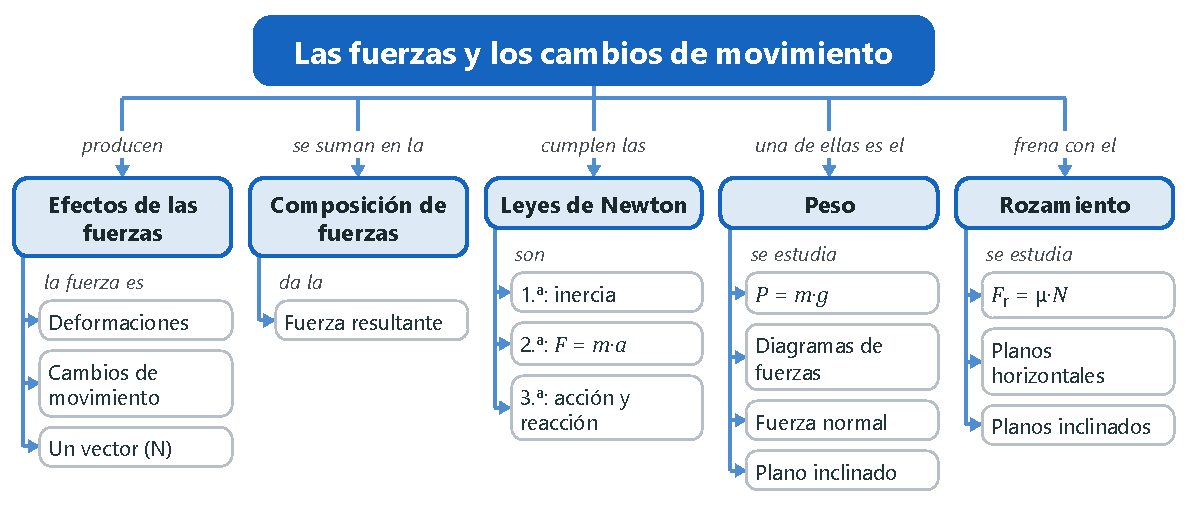
\includegraphics[width=\textwidth]{images/mapas_conceptuales/mapa_UD8}
\end{figure}

%========================================================================================
%\section*{Para empezar: aplicaciones de las leyes de la dinámica}
%\addcontentsline{toc}{section}{Para empezar: aplicaciones de las leyes de la dinámica}
%========================================================================================
%
%Si cuesta mucho poner en movimiento un cuerpo, también cuesta mucho detenerlo. Un gran petrolero cargado que navega a \qty{12}{\m\per\s} necesita \textbf{varios kilómetros} para pararse, porque tiende a mantener su estado de movimiento.
%
%En una lancha motora, la hélice empuja el agua hacia atrás y el agua, a su vez, empuja la lancha hacia delante. Mientras esa fuerza sea mayor que el rozamiento con el agua, la lancha acelera.
%
%Los fabricantes de zapatillas deportivas y de neumáticos invierten mucho dinero en diseñar productos que se agarren bien al suelo en cualquier situación. Por ejemplo, los dibujos de los neumáticos están pensados para que, cuando llueve, expulsen el agua y la rueda no pierda el contacto con el asfalto (\emph{aquaplaning}).
%
%Mejorar el agarre de los vehículos, y con ello la seguridad vial, tiene que ver con el \textbf{ODS 3} (\emph{Salud y bienestar}), cuya meta 3.6 es reducir las muertes y lesiones por accidentes de tráfico, y con el \textbf{ODS 11} (\emph{Ciudades y comunidades sostenibles}), que busca mejorar los sistemas de transporte.
%
%\begin{exercise}
%    La inercia es la tendencia de los cuerpos a mantener su estado de reposo o de movimiento. ¿Qué tiene que ver con que un petrolero necesite varios kilómetros para detenerse?
%    \begin{solu}
%        El petrolero tiene una masa enorme y, por tanto, mucha \textcolor{red}{inercia}: tiende a seguir moviéndose. Para frenarlo hace falta una fuerza que actúe durante mucho tiempo y a lo largo de mucha distancia.
%    \end{solu}
%\end{exercise}
%
%\begin{exercise}
%    Según el principio de acción y reacción, cuando dos cuerpos interaccionan, las fuerzas que se ejercen tienen igual módulo y dirección pero sentidos opuestos. ¿Cómo explica este principio el movimiento de la lancha?
%    \begin{solu}
%        La hélice empuja el agua hacia atrás (\textcolor{red}{acción}) y el agua empuja la hélice, y con ella la lancha, hacia delante (\textcolor{red}{reacción}).
%    \end{solu}
%\end{exercise}
%
%\begin{exercise}
%    ¿Para qué sirve el dibujo de la suela de las zapatillas de deporte? ¿Usarías un calzado con la suela lisa para hacer deporte? ¿Y por qué los neumáticos tienen dibujo?
%    \begin{solu}
%        El dibujo aumenta el \textcolor{red}{rozamiento} con el suelo y evita resbalar; con una suela lisa resbalaríamos con facilidad, sobre todo si el suelo está mojado. El dibujo de los neumáticos, además, \textcolor{red}{evacua el agua} cuando llueve para que la rueda siga en contacto con el asfalto.
%    \end{solu}
%\end{exercise}
%
%\begin{exercise}
%    En las carreras de coches, ¿se usan los mismos neumáticos con el asfalto seco que con el asfalto mojado? Investiga y relaciona tu respuesta con la seguridad vial y los ODS 3 y 11.
%    \begin{solu}
%        Respuesta libre. \textcolor{red}{No}: con el asfalto seco se usan neumáticos lisos (\emph{slicks}), que tienen más superficie en contacto con el suelo; con lluvia se usan neumáticos con surcos para evacuar el agua. Mejorar el agarre reduce los accidentes (ODS 3) y hace más seguro el transporte (ODS 11).
%    \end{solu}
%\end{exercise}

%========================================================================================
\section{¿Qué efectos producen las fuerzas?}
%========================================================================================

A nuestro alrededor vemos muchos efectos de las fuerzas: un muelle se estira o se encoge, un imán atrae un clavo, un balón se pone en movimiento o se detiene al golpearlo, una pelota deforma la red de la portería\ldots{} En todos los casos, la fuerza es una \textbf{interacción entre dos cuerpos}.

\begin{definition}[Fuerza]
    Una \textbf{fuerza} es toda causa capaz de modificar el estado de reposo o de movimiento de un cuerpo, o de producir en él una deformación. Su unidad en el SI es el \textbf{newton} (\unit{\newton}) y se mide con un \textbf{dinamómetro}.
\end{definition}

\subsection{La fuerza es una magnitud vectorial}

Para describir una fuerza no basta con su valor: no es lo mismo empujar una caja hacia la derecha que hacia arriba. La fuerza es un \textbf{vector} y tiene (figura~\ref{fig:vector_fuerza}):
\begin{itemize}
    \item \textbf{Punto de aplicación}: el lugar donde se aplica.
    \item \textbf{Módulo} o intensidad: su valor numérico, en newtons.
    \item \textbf{Dirección}: la de la recta sobre la que actúa.
    \item \textbf{Sentido}: el que indica la punta de la flecha.
\end{itemize}

\begin{figure}[H]
    \centering
    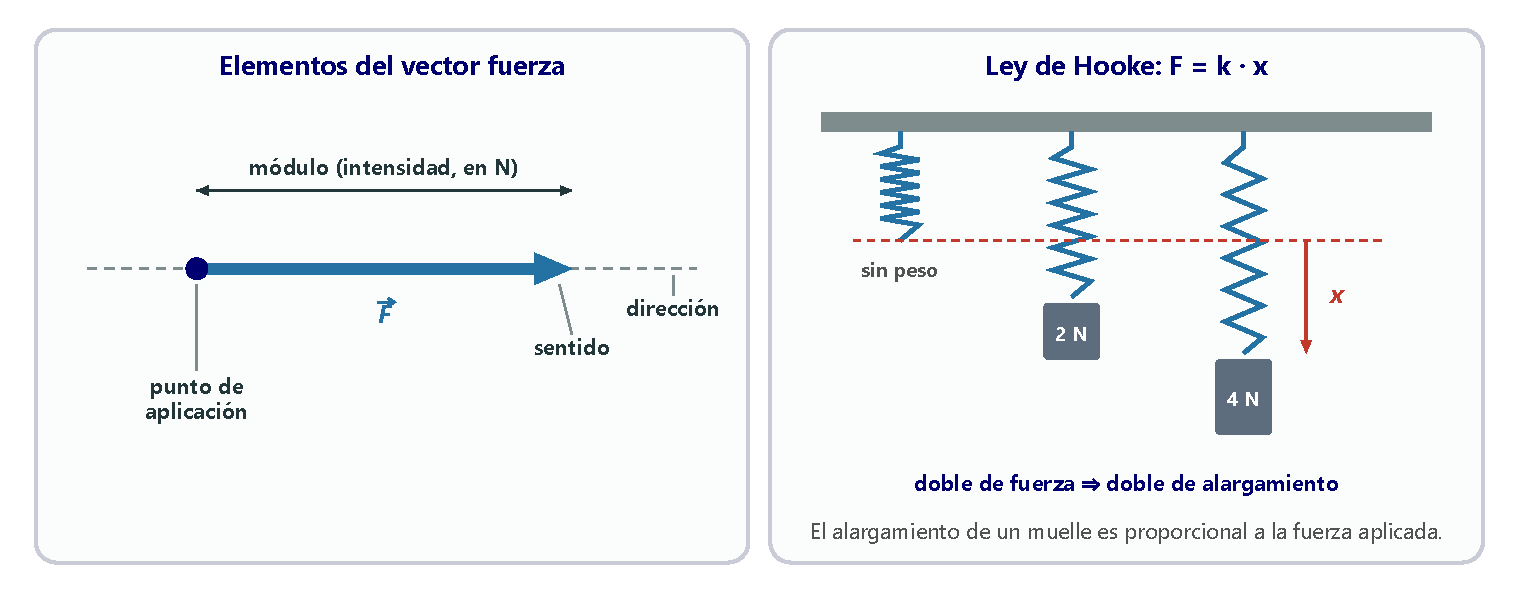
\includegraphics[width=\textwidth]{images/UD8/vector_fuerza}
    \caption{Elementos de una fuerza y ley de Hooke.}
    \label{fig:vector_fuerza}
\end{figure}

\begin{remark}
    \textbf{Ley de Hooke.} El alargamiento \(x\) que sufre un cuerpo elástico, como un muelle, es directamente proporcional a la fuerza \(F\) que lo produce: \(F = k \cdot x\). La constante \(k\), que se mide en \unit{\newton\per\m}, depende de cada muelle. En esta ley se basan los dinamómetros.
\end{remark}

\begin{exercise}
    En un partido de voleibol playa, las jugadoras golpean el balón hacia arriba; después el balón cae al otro lado de la red o, si choca con ella, la deforma. Analiza en cada situación si la fuerza cambia el estado de reposo o de movimiento del balón o produce una deformación.
    \begin{solu}
        Al golpear el balón, la fuerza \textcolor{red}{cambia su estado de movimiento} (su velocidad y su dirección) y lo \textcolor{red}{deforma} durante un instante. La gravedad cambia su movimiento haciéndolo caer. Al chocar con la red, el balón \textcolor{red}{se frena} y la red \textcolor{red}{se deforma}.
    \end{solu}
\end{exercise}

\begin{exercise}
    Cita dos ejemplos de fuerzas que deformen un cuerpo (de manera permanente o no) y dos en los que una fuerza cambie el estado de reposo o de movimiento de un cuerpo.
    \begin{solu}
        Respuesta libre. Deformaciones: estirar una goma elástica (no permanente), aplastar una lata (permanente). Cambio de movimiento: chutar un balón parado, frenar una bicicleta.
    \end{solu}
\end{exercise}

\begin{exercise}
    Un muelle se alarga \qty{4}{\cm} cuando le colgamos un peso de \qty{2}{\newton}.
    \begin{enumerate}[label=\alph*)]
        \item ¿Cuál es su constante elástica?
        \item ¿Cuánto se alargará con un peso de \qty{5}{\newton}?
    \end{enumerate}
    \begin{solu}
        a) \(k = \frac{F}{x} = \frac{2}{\num{0.04}} = \textcolor{red}{\qty{50}{\newton\per\m}}\). b) \(x = \frac{F}{k} = \frac{5}{50} = \qty{0.1}{\m} = \textcolor{red}{\qty{10}{\cm}}\).
    \end{solu}
\end{exercise}

\begin{exercise}
    Dibuja en unos ejes de coordenadas, con origen en el origen de coordenadas, una fuerza de \qty{3}{\newton} en el sentido positivo del eje X y otra de \qty{5}{\newton} en el sentido negativo del eje Y. Dibuja también las fuerzas opuestas a ellas y describe sus elementos.
    \begin{solu}
        Las cuatro tienen el punto de aplicación en O. \(\vec{F}_1\): módulo \qty{3}{\newton}, dirección del eje X, sentido positivo. \(\vec{F}_2\): módulo \qty{5}{\newton}, dirección del eje Y, sentido negativo. Sus opuestas tienen el \textcolor{red}{mismo módulo y dirección} pero \textcolor{red}{sentido contrario}: \qty{3}{\newton} hacia el X negativo y \qty{5}{\newton} hacia el Y positivo.
    \end{solu}
\end{exercise}

%========================================================================================
\section{¿Qué ocurre cuando actúan varias fuerzas? Composición de fuerzas}
%========================================================================================

Cuando varias fuerzas actúan a la vez sobre un cuerpo forman un \textbf{sistema de fuerzas}. Se llama \textbf{fuerza resultante}, \(\vec{R}\), a la fuerza que produce por sí sola el mismo efecto que todas ellas juntas.

\begin{definition}[Equilibrio]
    Un cuerpo está en \textbf{equilibrio} cuando está en reposo o se mueve con MRU. Para ello, la \textbf{resultante} de todas las fuerzas que actúan sobre él debe ser \textbf{nula}.
\end{definition}

\begin{figure}[H]
    \centering
    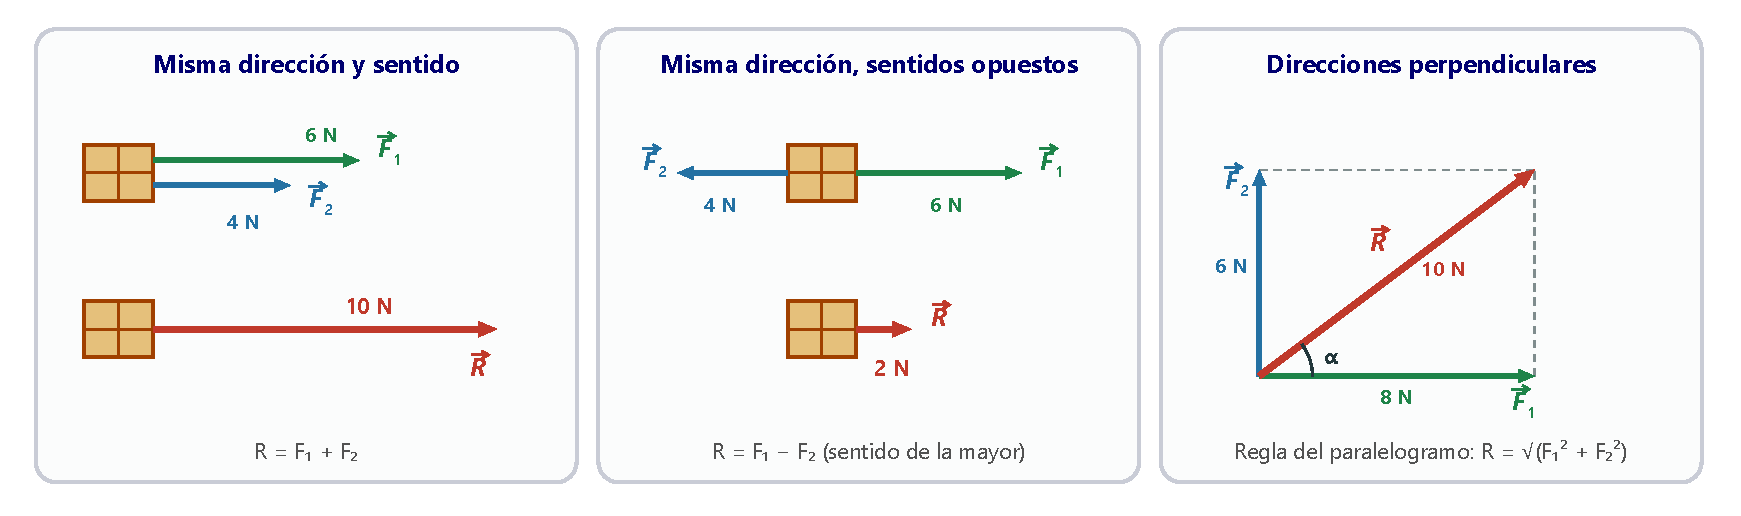
\includegraphics[width=\textwidth]{images/UD8/composicion_fuerzas}
    \caption{Resultante de dos fuerzas en tres casos.}
    \label{fig:composicion_fuerzas}
\end{figure}

\begin{itemize}
    \item \textbf{Misma dirección y sentido.} La resultante tiene la misma dirección y sentido, y su módulo es la \textbf{suma}: \(R = F_1 + F_2\).
    \item \textbf{Misma dirección y sentidos opuestos.} La resultante tiene la misma dirección, el sentido de la fuerza mayor y su módulo es la \textbf{diferencia}: \(R = F_1 - F_2\).
    \item \textbf{Direcciones perpendiculares.} Se aplica la \textbf{regla del paralelogramo}: se trazan por el extremo de cada fuerza paralelas a la otra; la resultante es la diagonal del paralelogramo. Su módulo se calcula con el teorema de Pitágoras y el ángulo con el eje X, con la trigonometría:
    \[ R = \sqrt{F_1^2 + F_2^2} \qquad \cos\alpha = \frac{F_1}{R} \qquad \sin\alpha = \frac{F_2}{R} \]
\end{itemize}

Para que un cuerpo sobre el que actúa una resultante \(\vec{R}\) quede en equilibrio hay que aplicarle otra fuerza, la \textbf{equilibrante}, del mismo módulo y dirección pero de sentido contrario.

\begin{example}
    Calcula la resultante de dos fuerzas perpendiculares de \qty{8}{\newton} (eje X) y \qty{6}{\newton} (eje Y) aplicadas en el mismo punto y el ángulo que forma con el eje X.
    \[ R = \sqrt{8^2 + 6^2} = \sqrt{100} = \textcolor{red}{\qty{10}{\newton}}; \qquad \cos\alpha = \frac{8}{10} = \num{0.8} \;\Rightarrow\; \alpha = \textcolor{red}{\ang{36.87}} \]
\end{example}

\begin{exercise}
    Dos fuerzas de la misma dirección y sentido, de \qty{12}{\newton} y \qty{9}{\newton}, actúan sobre un cuerpo.
    \begin{enumerate}[label=\alph*)]
        \item Calcula la resultante.
        \item ¿Qué fuerza habría que aplicar para equilibrarlas?
    \end{enumerate}
    \begin{solu}
        a) \(R = 12 + 9 = \textcolor{red}{\qty{21}{\newton}}\), con la misma dirección y sentido. b) Una fuerza de \textcolor{red}{\qty{21}{\newton}} con la misma dirección y \textcolor{red}{sentido contrario}.
    \end{solu}
\end{exercise}

\begin{exercise}
    Calcula la resultante de dos fuerzas de \qty{5}{\newton} y \qty{2}{\newton} con la misma dirección y sentidos contrarios.
    \begin{solu}
        \(R = 5 - 2 = \textcolor{red}{\qty{3}{\newton}}\), con la dirección común y el sentido de la fuerza de \qty{5}{\newton}.
    \end{solu}
\end{exercise}

\begin{exercise}
    Determina gráfica y numéricamente la resultante de dos fuerzas perpendiculares de \qty{60}{\newton} cada una. ¿Qué ángulo forma con el eje X?
    \begin{solu}
        \(R = \sqrt{60^2 + 60^2} = \textcolor{red}{\qty{84.9}{\newton}}\); \(\cos\alpha = \frac{60}{\num{84.9}} = \num{0.707} \Rightarrow \alpha = \textcolor{red}{\ang{45}}\): es la diagonal de un cuadrado.
    \end{solu}
\end{exercise}

\begin{exercise}
    Determina la resultante de dos fuerzas perpendiculares de \qty{12}{\newton} (eje X) y \qty{9}{\newton} (eje Y) y el ángulo que forma con el eje X.
    \begin{solu}
        \(R = \sqrt{144 + 81} = \textcolor{red}{\qty{15}{\newton}}\); \(\cos\alpha = \frac{12}{15} = \num{0.8} \Rightarrow \alpha = \textcolor{red}{\ang{36.87}}\).
    \end{solu}
\end{exercise}

\begin{exercise}
    Una fuerza de \qty{100}{\newton} es la resultante de dos fuerzas perpendiculares, una de las cuales vale \qty{60}{\newton}. ¿Cuánto vale la otra?
    \begin{solu}
        \(R^2 = F_1^2 + F_2^2 \Rightarrow F_2 = \sqrt{100^2 - 60^2} = \sqrt{6400} = \textcolor{red}{\qty{80}{\newton}}\).
    \end{solu}
\end{exercise}

\begin{exercise}
    Un remero empuja una barca río arriba con una fuerza de \qty{750}{\newton}, y la corriente la empuja río abajo con \qty{300}{\newton}. ¿Cuál es la resultante?
    \begin{solu}
        \(R = 750 - 300 = \textcolor{red}{\qty{450}{\newton}}\), \textcolor{red}{río arriba}.
    \end{solu}
\end{exercise}

\begin{exercise}
    Dos fuerzas de \qty{15}{\newton} y \qty{7}{\newton} aplicadas en un mismo cuerpo y con la misma dirección dan unas veces una resultante de \qty{22}{\newton} y otras de \qty{8}{\newton}. ¿A qué se debe?
    \begin{solu}
        Si tienen el \textcolor{red}{mismo sentido}, se suman: \(15 + 7 = \qty{22}{\newton}\). Si tienen \textcolor{red}{sentidos opuestos}, se restan: \(15 - 7 = \qty{8}{\newton}\).
    \end{solu}
\end{exercise}

\begin{exercise}
    Dos fuerzas de \qty{4}{\newton} y \qty{8}{\newton} están aplicadas en el mismo punto. Calcula la resultante si:
    \begin{enumerate}[label=\alph*)]
        \item tienen la misma dirección y sentido;
        \item tienen la misma dirección y sentidos opuestos;
        \item son perpendiculares.
    \end{enumerate}
    ¿Qué fuerza equilibraría cada resultante?
    \begin{solu}
        a) \(R = \textcolor{red}{\qty{12}{\newton}}\). b) \(R = \textcolor{red}{\qty{4}{\newton}}\) en el sentido de la de \qty{8}{\newton}. c) \(R = \sqrt{16 + 64} = \textcolor{red}{\qty{8.94}{\newton}}\), que forma con la fuerza de \qty{8}{\newton} un ángulo de \ang{26.6} (\(\cos\alpha = \frac{8}{\num{8.94}}\)). En cada caso, la equilibrante es una fuerza del mismo módulo y dirección que la resultante y sentido contrario.
    \end{solu}
\end{exercise}

\begin{exercise}
    Calcula la resultante de dos fuerzas perpendiculares de \qty{8}{\newton} y \qty{15}{\newton} aplicadas a un cuerpo.
    \begin{solu}
        \(R = \sqrt{64 + 225} = \sqrt{289} = \textcolor{red}{\qty{17}{\newton}}\).
    \end{solu}
\end{exercise}

%========================================================================================
\section{Fuerzas y cambios de movimiento: las leyes de Newton}
%========================================================================================

La parte de la Física que estudia la relación entre las fuerzas y los cambios de movimiento se llama \textbf{dinámica}. Sus fundamentos son las tres leyes que publicó Isaac \textbf{Newton} en 1687.

\subsection{La primera ley de Newton o principio de inercia}

¿Si un cuerpo está en reposo, es que no actúa ninguna fuerza sobre él? No necesariamente: un bloque sobre el que tiran dos fuerzas iguales y opuestas sigue en reposo, porque la resultante es nula. ¿Y hace falta una fuerza para que un cuerpo siga moviéndose? Una bola que rueda por una superficie horizontal perfectamente lisa no cambiaría su velocidad ni su dirección, aunque no la empujara nadie. En cambio, en un plano inclinado, la bola acelera al bajar y se frena al subir, porque el peso actúa sobre ella.

\begin{definition}[Primera ley de Newton o principio de inercia]
    Si sobre un cuerpo no actúa ninguna fuerza neta, el cuerpo permanece en \textbf{reposo} o se mueve con \textbf{movimiento rectilíneo y uniforme}. La \textbf{inercia} es la tendencia de los cuerpos a mantener su estado de reposo o de movimiento.
\end{definition}

Según el principio de inercia, el reposo y el MRU son equivalentes. Si un cuerpo acelera, frena o cambia de dirección, es que sobre él actúa una fuerza neta.

\begin{exercise}
    Indica si son verdaderas o falsas:
    \begin{enumerate}[label=\alph*)]
        \item si actúa una fuerza sobre un cuerpo, este tiene que cambiar su estado de reposo o de MRU;
        \item si no actúa ninguna fuerza sobre un cuerpo, este se mantiene en reposo o con MRU.
    \end{enumerate}
    \begin{solu}
        a) \textcolor{red}{Falsa}: si actúan varias fuerzas cuya resultante es nula, el estado no cambia. Lo correcto es decir «si actúa una fuerza \emph{neta}». b) \textcolor{red}{Verdadera}: es el principio de inercia.
    \end{solu}
\end{exercise}

\begin{exercise}
    Tapa un vaso con un naipe y pon una moneda encima. Si golpeas el naipe con fuerza en horizontal, ¿dónde cae la moneda? Justifícalo.
    \begin{solu}
        La moneda cae \textcolor{red}{dentro del vaso}. Por la \textcolor{red}{inercia}, tiende a seguir en reposo: el naipe sale disparado sin apenas arrastrarla, y la moneda, al quedarse sin apoyo, cae.
    \end{solu}
\end{exercise}

\begin{exercise}
    Cuando un coche frena bruscamente, los pasajeros siguen moviéndose hacia delante por la inercia; el cinturón de seguridad lo impide.
    \begin{enumerate}[label=\alph*)]
        \item ¿Para qué sirve el reposacabezas?
        \item ¿Por qué sientes que te empujan hacia atrás cuando el coche arranca bruscamente?
    \end{enumerate}
    \begin{solu}
        a) Si el coche recibe un golpe por detrás y acelera bruscamente, la cabeza tiende a quedarse donde estaba (inercia) y se iría hacia atrás: el reposacabezas la sujeta y evita lesiones en el cuello. b) Porque tu cuerpo tiende a seguir en reposo mientras el asiento avanza: en realidad no hay ninguna fuerza que te empuje hacia atrás, es el asiento el que te empuja hacia delante.
    \end{solu}
\end{exercise}

\begin{exercise}
    ¿Qué fuerza neta actúa sobre un coche que circula en línea recta a \qty{100}{\km\per\hour} constantes?
    \begin{solu}
        \textcolor{red}{Ninguna}: si se mueve con MRU, la fuerza neta es \textcolor{red}{nula}. La fuerza del motor compensa exactamente los rozamientos.
    \end{solu}
\end{exercise}

\subsection{La segunda ley de Newton o principio fundamental de la dinámica}

Si sobre un cuerpo actúa una fuerza neta, el cuerpo adquiere una aceleración. Para estudiarlo, colocamos un carrito en un carril, tiramos de él con distintas fuerzas (poniendo pesas en un portapesas) y medimos su aceleración a partir del tiempo que tarda en recorrer una distancia (\(a = 2s/t^2\)):

\begin{center}
    % --- tabla antigua ---
    % \begin{tblr}{colspec={lccccc}, hlines, vlines, column{1}={bg=ocre!85, fg=white, font=\bfseries}}
        % \(F\) (\unit{\newton}) & 2 & 3 & 4 & 5 & 6 \\
        % \(a\) (\unit{\m\per\square\s}) & \num{1.0} & \num{1.5} & \num{2.0} & \num{2.5} & \num{3.0} \\
    % \end{tblr}
    % --- tabla nueva ---
    \begin{tabular}{@{}lccccc@{}}
        \toprule
        \textbf{\(F\) (\unit{\newton})} & 2 & 3 & 4 & 5 & 6 \\[3pt]
        \textbf{\(a\) (\unit{\m\per\square\s})} & \num{1.0} & \num{1.5} & \num{2.0} & \num{2.5} & \num{3.0} \\
        \bottomrule
    \end{tabular}
    \qquad
    \begin{tikzpicture}[baseline=(current bounding box.center)]
        \begin{axis}[grafica, width=6cm, height=4.5cm, xlabel={\(a\) (\unit{\m\per\square\s})}, ylabel={\(F\) (\unit{\newton})}, xmin=0, xmax=3.3, ymin=0, ymax=7]
            \addplot coordinates {(1,2) (1.5,3) (2,4) (2.5,5) (3,6)};
            \addplot[mark=none, dashed, line width=0.8pt] coordinates {(0,0) (1,2)};
        \end{axis}
    \end{tikzpicture}
\end{center}

El cociente \(F/a\) es siempre el mismo, \qty{2}{\kg}: es la \textbf{masa} del carrito, que mide su \textbf{inercia}, es decir, lo que cuesta cambiar su estado de movimiento.

\begin{definition}[Segunda ley de Newton]
    La aceleración de un cuerpo es directamente proporcional a la fuerza neta que actúa sobre él, tiene su misma dirección y sentido, y es inversamente proporcional a su masa:
    \[ \vec{F}_\text{neta} = m \cdot \vec{a} \]
    Un \textbf{newton} es la fuerza que comunica a \qty{1}{\kg} de masa una aceleración de \qty{1}{\m\per\square\s}: \(\qty{1}{\newton} = \qty{1}{\kg\cdot\m\per\square\s}\).
\end{definition}

\begin{itemize}
    \item Si \(F_\text{neta} = 0\), la aceleración es nula: el cuerpo está en reposo o con MRU (primera ley).
    \item Si la fuerza neta tiene el sentido del movimiento, el cuerpo describe un \textbf{MRUA}.
    \item Si tiene sentido contrario al movimiento, el cuerpo describe un \textbf{MRUR} hasta pararse.
    \item Si es perpendicular al movimiento, el cuerpo \textbf{cambia de dirección}.
\end{itemize}

\begin{example}
    ¿Qué fuerza horizontal hay que aplicar a un cuerpo de \qty{40}{\kg} en reposo sobre un plano horizontal sin rozamiento para que alcance \qty{54}{\km\per\hour} en 6 s?

    \textcolor{blue}{Aceleración (MRUA):} \(v = \qty{15}{\m\per\s}\); \(a = \dfrac{15 - 0}{6} = \qty{2.5}{\m\per\square\s}\).

    \textcolor{blue}{Segunda ley:} \(F = m \cdot a = 40 \cdot \num{2.5} = \textcolor{red}{\qty{100}{\newton}}\).
\end{example}

\begin{exercise}
    ¿Qué fuerza hay que aplicar al carrito del experimento (\(m = \qty{2}{\kg}\)) para que adquiera una aceleración de \qty{1.5}{\m\per\square\s}? ¿Y de \qty{2.5}{\m\per\square\s}?
    \begin{solu}
        \(F = 2 \cdot \num{1.5} = \textcolor{red}{\qty{3}{\newton}}\); \(F = 2 \cdot \num{2.5} = \textcolor{red}{\qty{5}{\newton}}\).
    \end{solu}
\end{exercise}

\begin{exercise}
    ¿Qué fuerza hay que aplicar a un cuerpo de masa \(2m\) para que tenga la misma aceleración que otro de masa \(m\) al que se aplica una fuerza \(F\)? ¿Y si además queremos que la aceleración sea el doble?
    \begin{solu}
        Con la misma aceleración: \(F' = 2m \cdot a = \textcolor{red}{2F}\). Con el doble de aceleración: \(F'' = 2m \cdot 2a = \textcolor{red}{4F}\).
    \end{solu}
\end{exercise}

\begin{exercise}
    Una misma fuerza aplicada a dos cuerpos produce en uno una aceleración de \qty{1.8}{\m\per\square\s} y en el otro de \qty{9}{\m\per\square\s}. ¿Qué relación hay entre sus masas?
    \begin{solu}
        \(m_1 \cdot \num{1.8} = m_2 \cdot 9 \Rightarrow \frac{m_1}{m_2} = \frac{9}{\num{1.8}} = \textcolor{red}{5}\): el primero tiene \textcolor{red}{5 veces más masa}.
    \end{solu}
\end{exercise}

\begin{exercise}
    Un coche de \qty{1200}{\kg} parte del reposo empujado por una fuerza neta de \qty{2400}{\newton} en una carretera recta y horizontal. ¿Qué velocidad tendrá a los 10 s? ¿Qué espacio habrá recorrido?
    \begin{solu}
        \(a = \frac{2400}{1200} = \qty{2}{\m\per\square\s}\); \(v = 2 \cdot 10 = \textcolor{red}{\qty{20}{\m\per\s}}\); \(s = \frac{1}{2} \cdot 2 \cdot 10^2 = \textcolor{red}{\qty{100}{\m}}\).
    \end{solu}
\end{exercise}

\begin{exercise}
    Un coche de \qty{1200}{\kg} circula a \qty{72}{\km\per\hour}. ¿Qué fuerza deben ejercer los frenos para detenerlo en \qty{80}{\m}?
    \begin{solu}
        \(v_0 = \qty{20}{\m\per\s}\). \(0 - 20^2 = 2\,a \cdot 80 \Rightarrow a = \qty{-2.5}{\m\per\square\s}\); \(F = 1200 \cdot \num{2.5} = \textcolor{red}{\qty{3000}{\newton}}\), en sentido contrario al movimiento.
    \end{solu}
\end{exercise}

\begin{exercise}
    Un camión de 15 toneladas pasa de \qty{54}{\km\per\hour} a \qty{90}{\km\per\hour} en 50 s por una carretera horizontal. Calcula la fuerza neta, supuesta constante.
    \begin{solu}
        \(a = \frac{25 - 15}{50} = \qty{0.2}{\m\per\square\s}\); \(F = 15000 \cdot \num{0.2} = \textcolor{red}{\qty{3000}{\newton}}\).
    \end{solu}
\end{exercise}

\begin{exercise}
    ¿Qué fuerza horizontal constante hay que aplicar a un cuerpo de \qty{4}{\kg} en reposo sobre un plano horizontal sin rozamiento para que alcance \qty{18}{\km\per\hour} en 2 s?
    \begin{solu}
        \(a = \frac{5}{2} = \qty{2.5}{\m\per\square\s}\); \(F = 4 \cdot \num{2.5} = \textcolor{red}{\qty{10}{\newton}}\).
    \end{solu}
\end{exercise}

\subsection{La tercera ley de Newton o principio de acción y reacción}

Cuando una bola de billar choca de frente con otra en reposo, las dos se mueven después del choque. Si dos patinadores en reposo sobre el hielo se empujan, los dos salen despedidos en sentidos contrarios. Las fuerzas aparecen siempre como resultado de una \textbf{interacción} entre dos cuerpos: un cuerpo no puede ejercer ni sufrir una fuerza por sí solo.

\begin{definition}[Tercera ley de Newton]
    Cuando dos cuerpos interaccionan, las fuerzas que se ejercen el uno sobre el otro tienen el \textbf{mismo módulo y la misma dirección}, pero \textbf{sentidos opuestos}. Estas fuerzas de \textbf{acción y reacción} están aplicadas sobre \textbf{cuerpos diferentes}, por eso no se anulan entre sí.
\end{definition}

\begin{figure}[H]
    \centering
    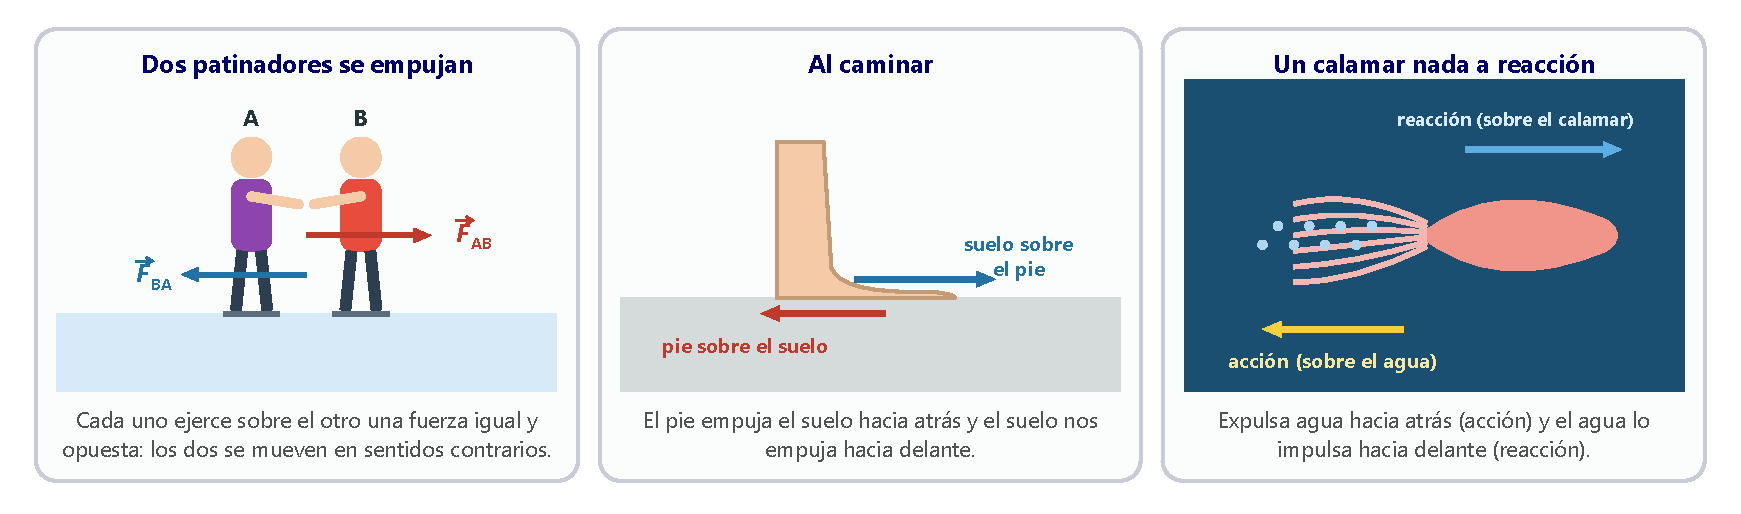
\includegraphics[width=\textwidth]{images/UD8/accion_reaccion}
    \caption{Ejemplos de parejas de fuerzas de acción y reacción.}
    \label{fig:accion_reaccion}
\end{figure}

Al caminar empujamos el suelo hacia atrás y el suelo nos empuja hacia delante; no vemos moverse la Tierra porque su masa es enorme. Al saltar de una barca al embarcadero, empujamos la barca hacia atrás y la barca nos empuja hacia delante.

\begin{example}
    \textbf{Las tres leyes al tirar de una maleta con ruedas.} \emph{Primera ley}: la maleta parada tiende a seguir en reposo, así que hay que tirar con una fuerza mayor que el rozamiento. \emph{Segunda ley}: mientras hay fuerza neta, la maleta acelera. Cuando tiramos justo con la fuerza que compensa el rozamiento, la fuerza neta es nula y la maleta sigue a velocidad constante (primera ley). \emph{Tercera ley}: la maleta tira de nosotros con una fuerza igual y opuesta a la nuestra; no se anulan porque actúan sobre cuerpos distintos.
\end{example}

\begin{exercise}
    Un estudiante razona: «Según la tercera ley de Newton, si tiro de una maleta, la maleta tira de mí con la misma fuerza en sentido opuesto; las dos fuerzas se anulan y nunca podré moverla». ¿Dónde está el error?
    \begin{solu}
        Las fuerzas de acción y reacción \textcolor{red}{actúan sobre cuerpos distintos} (una sobre la maleta y otra sobre el estudiante), así que \textcolor{red}{no se anulan}. Para saber si la maleta se mueve hay que fijarse solo en las fuerzas que actúan \emph{sobre la maleta}: nuestra fuerza y el rozamiento.
    \end{solu}
\end{exercise}

\begin{exercise}
    Un chico y una chica patinan sobre hielo unidos por una cuerda. El chico, de \qty{60}{\kg}, tira de la chica, de \qty{40}{\kg}, con una fuerza de \qty{12}{\newton}.
    \begin{enumerate}[label=\alph*)]
        \item ¿Qué aceleración adquiere la chica?
        \item ¿Qué fuerza actúa sobre el chico? ¿Qué aceleración adquiere él?
    \end{enumerate}
    \begin{solu}
        a) \(a = \frac{12}{40} = \textcolor{red}{\qty{0.3}{\m\per\square\s}}\). b) Por la tercera ley, la chica tira del chico con \textcolor{red}{\qty{12}{\newton}} en sentido contrario: \(a = \frac{12}{60} = \textcolor{red}{\qty{0.2}{\m\per\square\s}}\).
    \end{solu}
\end{exercise}

\begin{exercise}
    Cuando un caballo tira de un carro, los enganches están tirantes mientras el carro acelera, pero dejan de estarlo si se mueve a velocidad constante. Explícalo con las leyes de Newton.
    \begin{solu}
        Mientras acelera, el caballo tiene que ejercer una fuerza mayor que el rozamiento para que haya fuerza neta (segunda ley): los enganches transmiten esa fuerza y están tirantes (y, por la tercera ley, el carro tira del caballo con la misma fuerza). A velocidad constante, la fuerza neta es nula (primera ley): el caballo solo compensa el pequeño rozamiento de las ruedas y los enganches casi no se tensan.
    \end{solu}
\end{exercise}

\begin{exercise}
    Indica si son verdaderas o falsas y justifícalo:
    \begin{enumerate}[label=\alph*)]
        \item las fuerzas de acción y reacción nunca se anulan porque sus direcciones son diferentes;
        \item la aceleración de un cuerpo tiene siempre la dirección y el sentido de la fuerza neta;
        \item si ninguna fuerza actúa sobre un cuerpo, este está en reposo.
    \end{enumerate}
    \begin{solu}
        a) \textcolor{red}{Falsa}: tienen la misma dirección; no se anulan porque actúan sobre cuerpos distintos. b) \textcolor{red}{Verdadera} (segunda ley). c) \textcolor{red}{Falsa}: puede estar en reposo \emph{o moverse con MRU}.
    \end{solu}
\end{exercise}

%========================================================================================
\section{Una fuerza llamada peso}
%========================================================================================

Todos los cuerpos de la superficie terrestre están sometidos a la atracción gravitatoria de la Tierra, que les comunica la aceleración de la gravedad, \(g = \qty{9.8}{\m\per\square\s}\).

\begin{definition}[Peso]
    El \textbf{peso} es la fuerza con la que la Tierra (u otro astro) atrae a un cuerpo. Se mide en newtons y su módulo es:
    \[ P = m \cdot g \]
\end{definition}

\textbf{No hay que confundir masa y peso.} La \textbf{masa} mide la cantidad de materia de un cuerpo, es una magnitud \textbf{escalar}, se mide en kilogramos con una balanza y es la misma en cualquier lugar. El \textbf{peso} es una fuerza, una magnitud \textbf{vectorial}, se mide en newtons con un dinamómetro y depende del valor de \(g\) en cada lugar. Como vector, el peso tiene:
\begin{itemize}
    \item \textbf{módulo}: \(P = m \cdot g\);
    \item \textbf{punto de aplicación}: el \textbf{centro de gravedad} del cuerpo;
    \item \textbf{dirección}: vertical;
    \item \textbf{sentido}: hacia el centro de la Tierra.
\end{itemize}

\subsection{¿Cómo se identifican las fuerzas que actúan sobre un cuerpo?}

\begin{figure}[H]
    \centering
    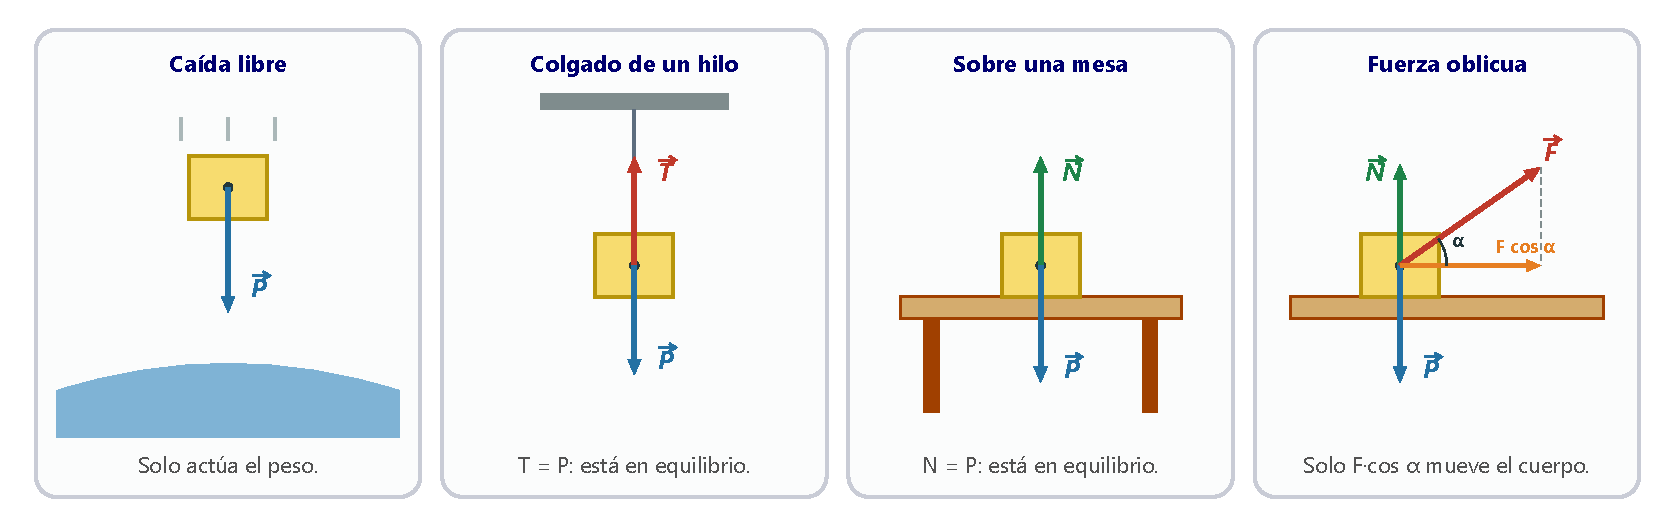
\includegraphics[width=\textwidth]{images/UD8/fuerzas_cuerpos}
    \caption{Fuerzas que actúan sobre un cuerpo en distintas situaciones.}
    \label{fig:fuerzas_cuerpos}
\end{figure}

\begin{itemize}
    \item \textbf{Cuerpo en caída libre.} Solo actúa el peso, \(\vec{P}\), aplicado en el centro de gravedad y dirigido hacia la Tierra. Su reacción, \(\vec{P}'\), es la fuerza con la que el cuerpo atrae a la Tierra, y está aplicada en ella.
    \item \textbf{Cuerpo colgado de un hilo.} Actúan el peso, \(\vec{P}\), y la \textbf{tensión} del hilo, \(\vec{T}\). Como el cuerpo está en reposo, \(T = P\). Sus reacciones son \(\vec{P}'\) (sobre la Tierra) y \(\vec{T}'\) (sobre el hilo).
    \item \textbf{Cuerpo apoyado en una superficie horizontal.} Actúan el peso, \(\vec{P}\), y la fuerza \textbf{normal}, \(\vec{N}\), que ejerce la superficie, perpendicular a ella. Como el cuerpo está en reposo, \(N = P\).
    \item \textbf{Si además empujamos horizontalmente con una fuerza \(F\)}, el peso y la normal se anulan y la fuerza neta es \(F\): \(a = \dfrac{F}{m}\) (sin rozamiento).
    \item \textbf{Si la fuerza forma un ángulo \(\alpha\) con la horizontal}, solo su componente horizontal, \(F \cos\alpha\), hace avanzar el cuerpo: \(a = \dfrac{F\cos\alpha}{m}\) (sin rozamiento).
\end{itemize}

\subsection{Cuerpo apoyado sobre un plano inclinado}

En un plano inclinado un ángulo \(\alpha\), el peso no es perpendicular a la superficie. Conviene descomponerlo en dos componentes (figura~\ref{fig:plano_inclinado}):
\begin{itemize}
    \item \(P_1 = P \sin\alpha = m\,g \sin\alpha\), paralela al plano y hacia abajo;
    \item \(P_2 = P \cos\alpha = m\,g \cos\alpha\), perpendicular al plano.
\end{itemize}
La normal solo equilibra a \(P_2\): \(N = m\,g\cos\alpha\). La componente \(P_1\) no está equilibrada y, si no hay rozamiento, hace bajar el cuerpo con aceleración:
\[ m\,g\sin\alpha = m\,a \;\Rightarrow\; a = g \sin\alpha \]
Esta aceleración solo depende del ángulo de inclinación, \textbf{no de la masa} del cuerpo.

\begin{figure}[H]
    \centering
    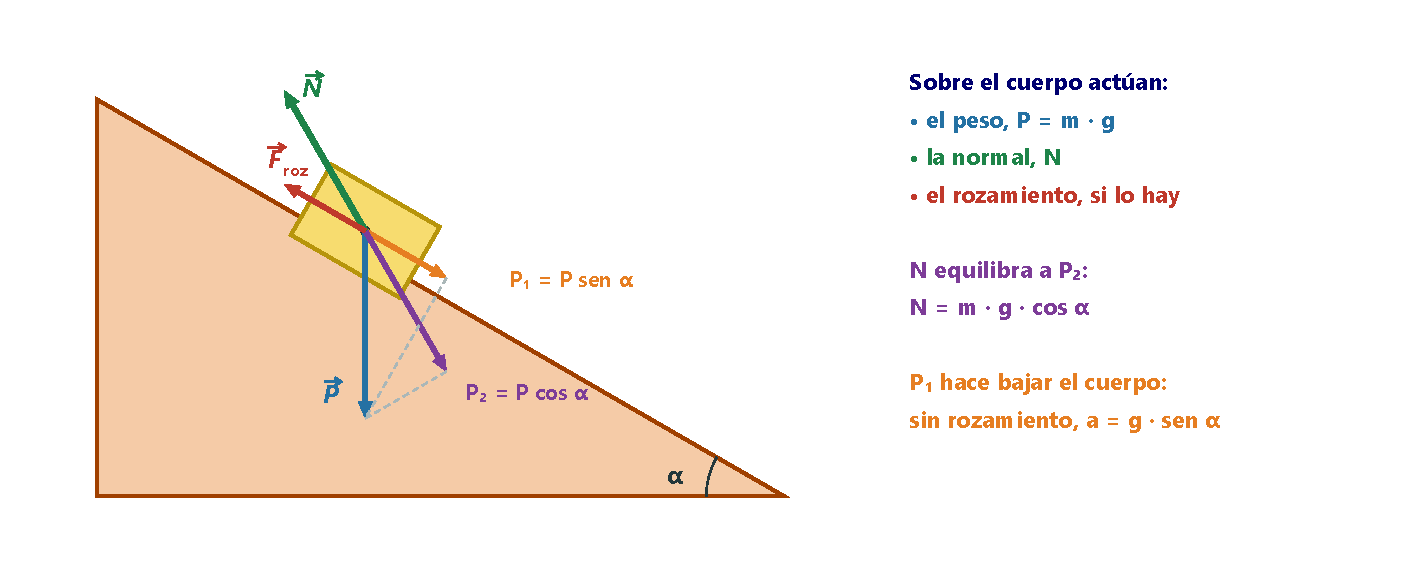
\includegraphics[width=0.9\textwidth]{images/UD8/plano_inclinado}
    \caption{Fuerzas sobre un cuerpo apoyado en un plano inclinado.}
    \label{fig:plano_inclinado}
\end{figure}

\begin{example}
    Calcula la aceleración con la que baja un cuerpo por un plano inclinado \ang{30} sin rozamiento.
    \[ a = g \sin\alpha = \num{9.8} \cdot \sin\ang{30} = \num{9.8} \cdot \num{0.5} = \textcolor{red}{\qty{4.9}{\m\per\square\s}} \]
\end{example}

\begin{exercise}
    ¿Cuánto pesa una persona de \qty{65}{\kg} en la Tierra (\(g = \qty{9.8}{\m\per\square\s}\))? ¿Y en la Luna (\(g = \qty{1.6}{\m\per\square\s}\))? ¿Cambia su masa?
    \begin{solu}
        Tierra: \(P = 65 \cdot \num{9.8} = \textcolor{red}{\qty{637}{\newton}}\). Luna: \(P = 65 \cdot \num{1.6} = \textcolor{red}{\qty{104}{\newton}}\). Su masa \textcolor{red}{no cambia}: es de \qty{65}{\kg} en los dos sitios.
    \end{solu}
\end{exercise}

\begin{exercise}
    Dibuja las fuerzas que actúan sobre un cuerpo de \qty{8}{\kg} colgado de un hilo. Calcula el peso y la tensión del hilo.
    \begin{solu}
        Actúan el peso, hacia abajo, y la tensión, hacia arriba (como en la figura~\ref{fig:fuerzas_cuerpos}). \(P = 8 \cdot \num{9.8} = \textcolor{red}{\qty{78.4}{\newton}}\); como está en equilibrio, \(T = P = \textcolor{red}{\qty{78.4}{\newton}}\).
    \end{solu}
\end{exercise}

\begin{exercise}
    Calcula la aceleración con la que baja un cuerpo por un plano inclinado \ang{45} sin rozamiento.
    \begin{solu}
        \(a = \num{9.8} \cdot \sin\ang{45} = \num{9.8} \cdot \num{0.707} = \textcolor{red}{\qty{6.93}{\m\per\square\s}}\).
    \end{solu}
\end{exercise}

\begin{exercise}
    Copia y completa la tabla para un cuerpo de \qty{50}{\kg}. ¿En qué lugar intentarías batir tu récord de salto de altura? ¿En cuál no lo intentarías nunca?
    \begin{center}
        % --- tabla antigua ---
        % \begin{tblr}{colspec={lcc}, hlines, vlines, row{1}={bg=ocre!85, fg=white, font=\bfseries}}
            % Lugar & Masa (\unit{\kg}) & Peso (\unit{\newton}) \\
            % Espacio lejos de los astros (\(g \approx 0\)) & 50 & \ldots \\
            % Superficie de la Tierra (\(g = \qty{9.8}{\m\per\square\s}\)) & 50 & \ldots \\
            % Superficie de la Luna (\(g = \qty{1.6}{\m\per\square\s}\)) & 50 & \ldots \\
            % Superficie de Júpiter (\(g = \qty{24.8}{\m\per\square\s}\)) & 50 & \ldots \\
        % \end{tblr}
        % --- tabla nueva ---
        \begin{tabular}{@{}lcc@{}}
            \toprule
            \textbf{Lugar} & \textbf{Masa (\unit{\kg})} & \textbf{Peso (\unit{\newton})} \\
            \midrule
            Espacio lejos de los astros (\(g \approx 0\)) & 50 & \ldots \\[3pt]
            Superficie de la Tierra (\(g = \qty{9.8}{\m\per\square\s}\)) & 50 & \ldots \\[3pt]
            Superficie de la Luna (\(g = \qty{1.6}{\m\per\square\s}\)) & 50 & \ldots \\[3pt]
            Superficie de Júpiter (\(g = \qty{24.8}{\m\per\square\s}\)) & 50 & \ldots \\
            \bottomrule
        \end{tabular}
    \end{center}
    \begin{solu}
        Pesos: \textcolor{red}{0}; \textcolor{red}{\qty{490}{\newton}}; \textcolor{red}{\qty{80}{\newton}}; \textcolor{red}{\qty{1240}{\newton}}. Intentaría batir el récord en la \textcolor{red}{Luna} (donde menos pesaría, aunque fuera de los astros no hay «suelo» del que saltar), y nunca en \textcolor{red}{Júpiter}.
    \end{solu}
\end{exercise}

\begin{exercise}
    Un astronauta está en un lugar del espacio donde la gravedad es la mitad que en la superficie terrestre. Indica si son verdaderas o falsas:
    \begin{enumerate}[label=\alph*)]
        \item su peso es el mismo que en la Tierra;
        \item su masa es el doble;
        \item allí pesa la mitad.
    \end{enumerate}
    \begin{solu}
        a) \textcolor{red}{Falsa}. b) \textcolor{red}{Falsa}: la masa no cambia. c) \textcolor{red}{Verdadera}: \(P = m \cdot \frac{g}{2}\).
    \end{solu}
\end{exercise}

\begin{exercise}
    Indica si son verdaderas o falsas y corrige las falsas:
    \begin{enumerate}[label=\alph*)]
        \item el peso es la cantidad de materia de un cuerpo;
        \item la masa se mide con una balanza comparándola con una masa patrón;
        \item el peso está aplicado en el centro de gravedad y dirigido hacia el centro de la Tierra;
        \item el peso de un cuerpo no depende del lugar donde se encuentre.
    \end{enumerate}
    \begin{solu}
        a) \textcolor{red}{Falsa}: eso es la masa; el peso es la fuerza con que la Tierra atrae al cuerpo. b) \textcolor{red}{Verdadera}. c) \textcolor{red}{Verdadera}. d) \textcolor{red}{Falsa}: depende del valor de \(g\) en ese lugar.
    \end{solu}
\end{exercise}

\begin{exercise}
    Dibuja las fuerzas que actúan sobre un cuerpo de \qty{10}{\kg} apoyado en una superficie horizontal sin rozamiento, al que se aplica una fuerza horizontal de \qty{20}{\newton}. ¿Con qué aceleración se mueve?
    \begin{solu}
        Actúan el peso (\qty{98}{\newton}, hacia abajo), la normal (\qty{98}{\newton}, hacia arriba) y la fuerza aplicada. Las dos primeras se anulan: \(a = \frac{20}{10} = \textcolor{red}{\qty{2}{\m\per\square\s}}\).
    \end{solu}
\end{exercise}

\begin{exercise}
    A un cuerpo de \qty{5}{\kg} apoyado en una superficie horizontal sin rozamiento se le aplica una fuerza de \qty{20}{\newton} que forma \ang{30} con la horizontal. ¿Con qué aceleración se mueve?
    \begin{solu}
        Solo la componente horizontal produce el movimiento: \(F\cos\ang{30} = 20 \cdot \num{0.866} = \qty{17.3}{\newton}\); \(a = \frac{\num{17.3}}{5} = \textcolor{red}{\qty{3.46}{\m\per\square\s}}\).
    \end{solu}
\end{exercise}

\begin{exercise}
    Un cuerpo de \qty{20}{\kg} apoyado en un plano inclinado \ang{30} sin rozamiento se empuja hacia arriba con una fuerza de \qty{200}{\newton} paralela al plano. ¿Con qué aceleración sube?
    \begin{solu}
        \(P_1 = 20 \cdot \num{9.8} \cdot \num{0.5} = \qty{98}{\newton}\) hacia abajo. \(F_\text{neta} = 200 - 98 = \qty{102}{\newton}\); \(a = \frac{102}{20} = \textcolor{red}{\qty{5.1}{\m\per\square\s}}\).
    \end{solu}
\end{exercise}

\begin{exercise}
    ¿Qué fuerza paralela al plano hay que aplicar a un cuerpo de \qty{10}{\kg} para que suba por un plano inclinado \ang{30} sin rozamiento con una aceleración de \qty{5.1}{\m\per\square\s}? ¿Y para que suba con velocidad constante?
    \begin{solu}
        \(F - m g \sin\ang{30} = m a \Rightarrow F = 10 \cdot \num{5.1} + 10 \cdot \num{9.8} \cdot \num{0.5} = 51 + 49 = \textcolor{red}{\qty{100}{\newton}}\). Con velocidad constante, \(a = 0\): \(F = m g \sin\alpha = \textcolor{red}{\qty{49}{\newton}}\).
    \end{solu}
\end{exercise}

%========================================================================================
\section{¿Por qué se paran los cuerpos? La fuerza de rozamiento}
%========================================================================================

Según la primera ley, un cuerpo con MRU debería seguir moviéndose indefinidamente; y, según la segunda, cualquier fuerza, por pequeña que sea, debería acelerarlo. Sin embargo, una pelota que rueda acaba parándose, y un mueble pesado no se mueve si lo empujamos suavemente. La causa es la \textbf{fuerza de rozamiento}.

\begin{definition}[Fuerza de rozamiento]
    Es la fuerza que aparece en la superficie de contacto entre dos cuerpos cuando uno se desliza, o tiende a deslizarse, sobre el otro. Es \textbf{paralela} a las superficies en contacto y de \textbf{sentido opuesto} al movimiento.
\end{definition}

\subsection{¿De qué depende la fuerza de rozamiento?}

Con un bloque sobre una mesa unido a un portapesas mediante un hilo y una polea, añadimos pesas hasta que el bloque empieza a deslizar (figura~\ref{fig:rozamiento_montaje}). En ese momento, la fuerza aplicada es igual a la de rozamiento. Así se comprueba que la fuerza de rozamiento:
\begin{itemize}
    \item depende de la \textbf{naturaleza} de las superficies en contacto y de su pulimento;
    \item \textbf{no depende del área} de las superficies en contacto (da igual sobre qué cara apoyemos el bloque);
    \item es \textbf{proporcional a la fuerza normal} con la que una superficie aprieta a la otra:
    \[ F_\text{roz} = \mu \cdot N \]
    donde \(\mu\) es el \textbf{coeficiente de rozamiento}, que no tiene unidades y depende de las superficies en contacto. Sobre una superficie horizontal, \(N = m\,g\) y \(F_\text{roz} = \mu\,m\,g\).
\end{itemize}

\begin{figure}[H]
    \centering
    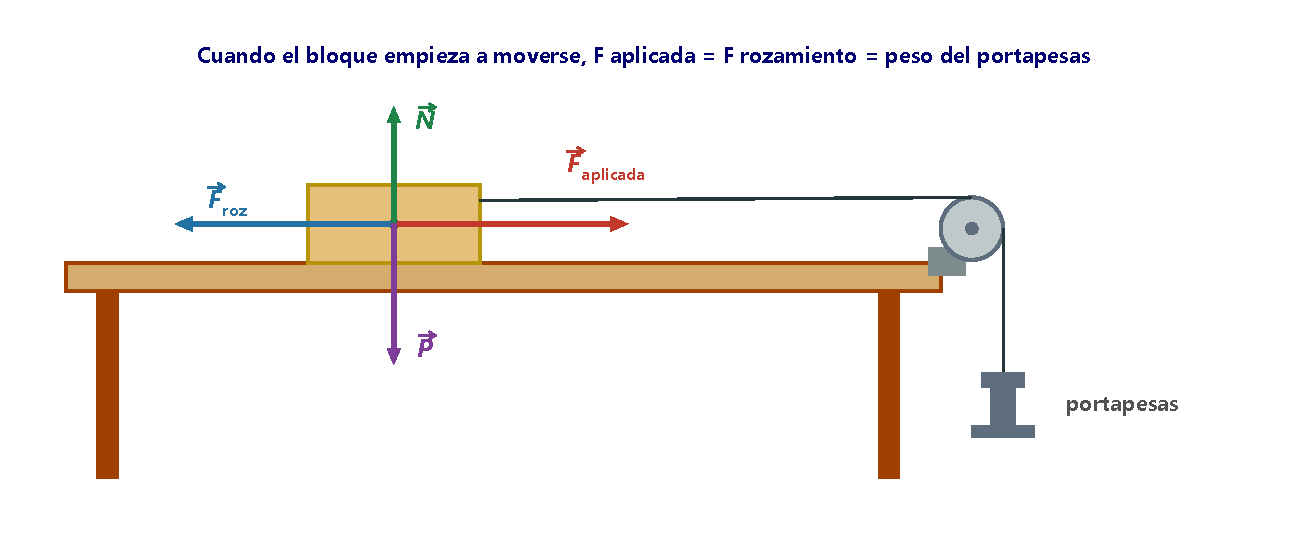
\includegraphics[width=0.85\textwidth]{images/UD8/rozamiento_montaje}
    \caption{Montaje para estudiar la fuerza de rozamiento.}
    \label{fig:rozamiento_montaje}
\end{figure}

\subsection{Problemas con rozamiento en planos horizontales e inclinados}

\begin{marker}
    \textbf{Cómo resolver problemas de dinámica.}
    \begin{enumerate}[label=\arabic*.]
        \item Haz un esquema de la situación.
        \item Dibuja todas las fuerzas que actúan sobre el cuerpo y calcula la fuerza neta en la dirección del movimiento.
        \item Aplica la segunda ley de Newton, \(F_\text{neta} = m \cdot a\), para calcular lo que se pide.
    \end{enumerate}
\end{marker}

\begin{example}
    ¿Qué fuerza horizontal hay que aplicar a un cuerpo de \qty{25}{\kg} para que se deslice con velocidad uniforme sobre una superficie horizontal, si \(\mu = \num{0.1}\)?

    Si la velocidad es constante, \(a = 0\) y la fuerza neta es nula: la fuerza aplicada es igual a la de rozamiento.
    \[ F = F_\text{roz} = \mu\,m\,g = \num{0.1} \cdot 25 \cdot \num{9.8} = \textcolor{red}{\qty{24.5}{\newton}} \]
\end{example}

\begin{example}
    A un cuerpo de \qty{4}{\kg} apoyado en un plano horizontal se le aplica una fuerza horizontal de \qty{40}{\newton}. Si \(\mu = \num{0.1}\), ¿qué aceleración adquiere?
    \[ F_\text{roz} = \num{0.1} \cdot 4 \cdot \num{9.8} = \qty{3.92}{\newton}; \quad F_\text{neta} = 40 - \num{3.92} = \qty{36.08}{\newton}; \quad a = \frac{\num{36.08}}{4} = \textcolor{red}{\qty{9.02}{\m\per\square\s}} \]
\end{example}

\begin{example}
    Un cuerpo baja por un plano inclinado \ang{30} bajo la acción de su peso. Si \(\mu = \num{0.2}\), ¿con qué aceleración lo hace?

    Ahora la fuerza neta es \(P_1 - F_\text{roz}\), con \(F_\text{roz} = \mu\,N = \mu\,m\,g\cos\alpha\):
    \[ m\,a = m\,g\sin\alpha - \mu\,m\,g\cos\alpha \;\Rightarrow\; a = \num{9.8}\,(\num{0.5} - \num{0.2} \cdot \num{0.866}) = \textcolor{red}{\qty{3.20}{\m\per\square\s}} \]
    Sin rozamiento serían \qty{4.9}{\m\per\square\s}.
\end{example}

\begin{exercise}
    Indica si son verdaderas o falsas y corrige las falsas. La fuerza de rozamiento\ldots
    \begin{enumerate}[label=\alph*)]
        \item se opone al movimiento;
        \item no depende del peso del cuerpo apoyado sobre una superficie horizontal;
        \item depende del área de las superficies en contacto;
        \item depende de la naturaleza de las superficies en contacto;
        \item tiene un coeficiente que se mide en newtons;
        \item no es un vector;
        \item es perpendicular a las superficies en contacto.
    \end{enumerate}
    \begin{solu}
        a) \textcolor{red}{Verdadera}. b) \textcolor{red}{Falsa}: sobre una superficie horizontal \(N = P\), así que es proporcional al peso. c) \textcolor{red}{Falsa}: no depende del área. d) \textcolor{red}{Verdadera}. e) \textcolor{red}{Falsa}: el coeficiente no tiene unidades. f) \textcolor{red}{Falsa}: es una fuerza y, por tanto, un vector. g) \textcolor{red}{Falsa}: es paralela a las superficies.
    \end{solu}
\end{exercise}

\begin{exercise}
    Un bloque de \qty{5}{\kg} está sobre una mesa (\(\mu = \num{0.1}\)) y tiramos de él horizontalmente con un dinamómetro. ¿Qué marcará el dinamómetro cuando el bloque empiece a deslizar?
    \begin{solu}
        \(F = \mu\,m\,g = \num{0.1} \cdot 5 \cdot \num{9.8} = \textcolor{red}{\qty{4.9}{\newton}}\).
    \end{solu}
\end{exercise}

\begin{exercise}
    ¿Qué fuerza hay que aplicar a un cuerpo de \qty{12}{\kg} para desplazarlo con velocidad uniforme sobre una superficie horizontal si \(\mu = \num{0.15}\)?
    \begin{solu}
        \(F = F_\text{roz} = \num{0.15} \cdot 12 \cdot \num{9.8} = \textcolor{red}{\qty{17.6}{\newton}}\).
    \end{solu}
\end{exercise}

\begin{exercise}
    ¿Qué fuerza horizontal hay que aplicar a un bloque de cemento de \qty{80}{\kg} para que se deslice con velocidad uniforme sobre una superficie horizontal, si \(\mu = \num{0.2}\)? Dibuja todas las fuerzas que actúan sobre el bloque.
    \begin{solu}
        Actúan el peso, la normal, la fuerza aplicada y el rozamiento (como en la figura~\ref{fig:rozamiento_montaje}). \(F = \num{0.2} \cdot 80 \cdot \num{9.8} = \textcolor{red}{\qty{156.8}{\newton}}\).
    \end{solu}
\end{exercise}

\begin{exercise}
    Calcula la fuerza de rozamiento sobre un bloque de \qty{15}{\kg} que se desliza por una superficie horizontal con \(\mu = \num{0.3}\). ¿Y sobre un bloque que pesa \qty{150}{\newton} si \(\mu = \num{0.2}\)?
    \begin{solu}
        \(F_\text{roz} = \num{0.3} \cdot 15 \cdot \num{9.8} = \textcolor{red}{\qty{44.1}{\newton}}\). \quad \(F_\text{roz} = \num{0.2} \cdot 150 = \textcolor{red}{\qty{30}{\newton}}\).
    \end{solu}
\end{exercise}

\begin{exercise}
    Se aplica una fuerza horizontal de \qty{36}{\newton} a un cuerpo de \qty{6}{\kg} que se desplaza por una superficie horizontal con \(\mu = \num{0.2}\). ¿Qué aceleración adquiere?
    \begin{solu}
        \(F_\text{roz} = \num{0.2} \cdot 6 \cdot \num{9.8} = \qty{11.76}{\newton}\); \(a = \frac{36 - \num{11.76}}{6} = \textcolor{red}{\qty{4.04}{\m\per\square\s}}\).
    \end{solu}
\end{exercise}

\begin{exercise}
    Sobre un cuerpo de \qty{8}{\kg} que se mueve por un plano horizontal se aplica una fuerza horizontal de \qty{60}{\newton}. Si \(\mu = \num{0.15}\), ¿qué aceleración adquiere?
    \begin{solu}
        \(F_\text{roz} = \num{0.15} \cdot 8 \cdot \num{9.8} = \qty{11.76}{\newton}\); \(a = \frac{60 - \num{11.76}}{8} = \textcolor{red}{\qty{6.03}{\m\per\square\s}}\).
    \end{solu}
\end{exercise}

\begin{exercise}
    ¿Qué fuerza horizontal hay que aplicar a un cuerpo de \qty{60}{\kg} para que se desplace con velocidad uniforme si \(\mu = \num{0.5}\)?
    \begin{solu}
        \(F = \num{0.5} \cdot 60 \cdot \num{9.8} = \textcolor{red}{\qty{294}{\newton}}\).
    \end{solu}
\end{exercise}

\begin{exercise}
    Un cuerpo baja por un plano inclinado \ang{45} bajo la acción de su peso. Halla su aceleración si \(\mu = \num{0.1}\). Dibuja las fuerzas que actúan sobre él.
    \begin{solu}
        Actúan el peso (descompuesto en \(P_1\) y \(P_2\)), la normal y el rozamiento hacia arriba del plano, como en la figura~\ref{fig:plano_inclinado}.
        \(a = g(\sin\ang{45} - \mu\cos\ang{45}) = \num{9.8}\,(\num{0.707} - \num{0.0707}) = \textcolor{red}{\qty{6.24}{\m\per\square\s}}\).
    \end{solu}
\end{exercise}

\begin{exercise}
    Un cuerpo baja por un plano inclinado \ang{30} bajo la acción de su peso. Halla su aceleración si \(\mu = \num{0.1}\).
    \begin{solu}
        \(a = \num{9.8}\,(\num{0.5} - \num{0.1} \cdot \num{0.866}) = \textcolor{red}{\qty{4.05}{\m\per\square\s}}\).
    \end{solu}
\end{exercise}

\begin{exercise}
    Un cuerpo de \qty{10}{\kg} baja por un plano inclinado \ang{45} con \(\mu = \num{0.1}\). ¿Qué fuerza paralela al plano hay que ejercer para que baje con velocidad constante?
    \begin{solu}
        Con velocidad constante, la fuerza neta es nula: \(F + F_\text{roz} = P_1\).
        \(P_1 = 98 \cdot \num{0.707} = \qty{69.3}{\newton}\); \(F_\text{roz} = \num{0.1} \cdot 98 \cdot \num{0.707} = \qty{6.93}{\newton}\); \(F = \num{69.3} - \num{6.93} = \textcolor{red}{\qty{62.4}{\newton}}\), dirigida \textcolor{red}{hacia arriba del plano}.
    \end{solu}
\end{exercise}

\begin{exercise}
    Calcula la aceleración con la que sube un cuerpo de \qty{10}{\kg} apoyado en un plano inclinado \ang{30} si se le empuja hacia arriba con una fuerza de \qty{200}{\newton} paralela al plano y \(\mu = \num{0.2}\).
    \begin{solu}
        Ahora el rozamiento actúa hacia abajo, como \(P_1\): \(P_1 = 98 \cdot \num{0.5} = \qty{49}{\newton}\); \(F_\text{roz} = \num{0.2} \cdot 98 \cdot \num{0.866} = \qty{16.97}{\newton}\).
        \(a = \frac{200 - 49 - \num{16.97}}{10} = \textcolor{red}{\qty{13.4}{\m\per\square\s}}\).
    \end{solu}
\end{exercise}
